\documentclass[aspectratio=169]{beamer}
\usetheme{Antibes}

\usepackage[magyar]{babel}
\usepackage[stixtwo]{fontsetup}

\usepackage{graphicx}

\usepackage{minted}

\title{Gépi látás házi feladat GL6}
\author{Molnár Ferenc Tamás (EOZV2E) \\ Sándor Tibor (C7XUDE) \\ Frikker Erik Vince (D3KKX6) \\ Klucsik Ákos (D6S9IZ) \\ Hajdu Ákos (HEP79U)}
\date{2025. május 11.}

\begin{document}

\frame{\titlepage}

\section{Bevezetés}
\begin{frame}
	\frametitle{Célkitűzések}

	\begin{itemize}
		\item Cél: Magyar rendszámmal rendelkező autók rendszámtáblájának
		      detektálása és a rajta lévő karakterek kiolvasása
		\item Rendelkezésre álló adatok:
		      \begin{itemize}
			      \item $\sim 1400$db képből álló adatbázis
			      \item Egy csv fájl, amely tartalmazza a képen szereplő autók
			            rendszámait
		      \end{itemize}
	\end{itemize}
\end{frame}

\begin{frame}
	\frametitle{Projekt felépítése}

	\begin{itemize}
		\item Rendszámtáblák detektálása: YOLOv8
		\item Rendszámtábla karakterek felismerése: fast-plate-ocr
		\item Használat:
		      \begin{itemize}
			      \item Mappában lévő képek detekciója
			      \item Webes felület: React, Backend: fastapi
		      \end{itemize}
	\end{itemize}
\end{frame}

\section{Megvalósítás}
\subsection{Rendszámtábla detekció}
\begin{frame}
	\frametitle{1. lépés: Képek egy részének annotálása}

	\centering
	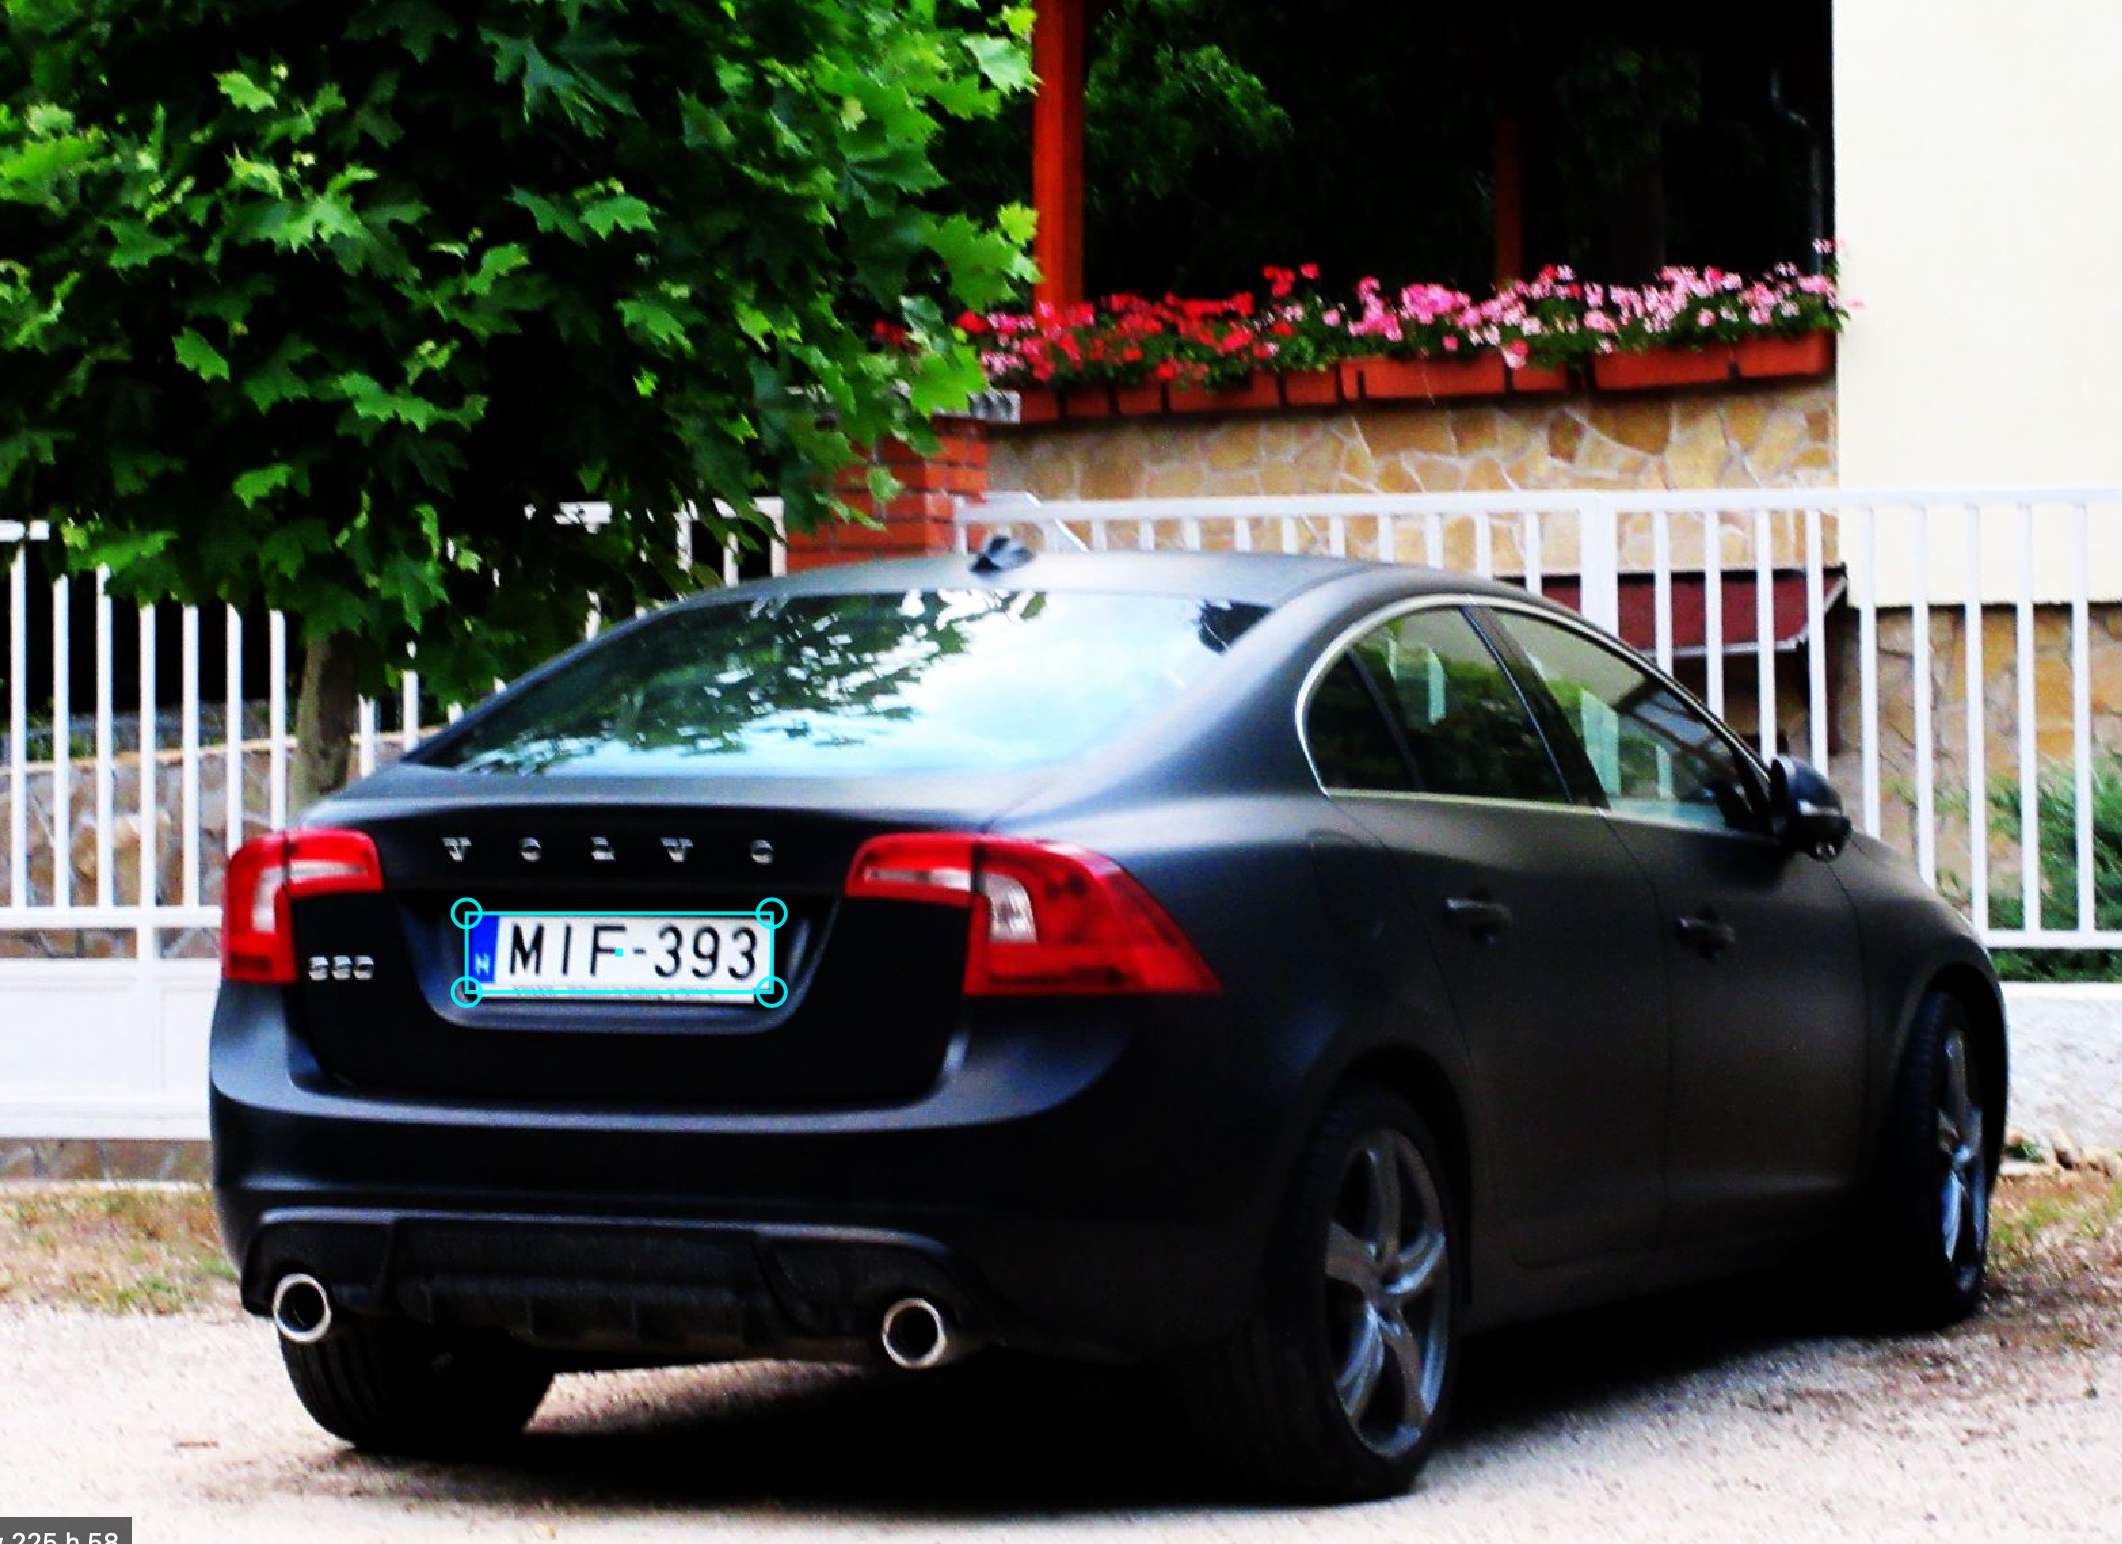
\includegraphics[width=0.55\textwidth]{images/01_manual.png}
\end{frame}

\begin{frame}[fragile]
	\frametitle{2. lépés: YOLO betanítása az annotált képekkel}

	\begin{minted}[fontsize=\footnotesize]{python}
model.train(
    data='datasets/data_manual.yaml', # konfigurációs fájl
    epochs=100,                       # epochok száma -> hányszor fut végig
    imgsz=512,                        # maximális kép méret -> gyorsabb betanítás
    batch=32,                         # batch méret -> egy lépésben feldolgozott képek
    device="mps",                     # GPU használata
    workers=8,                        # Szálak száma -> párhuzamos feldolgozás
    cache=True,                       # Képek cache-elése -> gyorsabb betanítás
    augment=True,                     # Augmentáció -> képek elforgatása, torzítása
    name='yolov8n_manual_train',      # Modell neve
    optimizer='AdamW',                # Optimalizáló algoritmus -> súlycsökkentéssel
    lr0=1e-3,                         # Kezdeti tanulási ráta
    lrf=0.01,                         # Tanulási ráta csökkentése a végén
    weight_decay=1e-2,                # Súlycsökkentés -> túlillesztést gátolja
    patience=10,                      # Túlillesztés gátlás
    seed=42,                          # Véletlenszám generátor magja -> reprodukálhatóság
)
\end{minted}
\end{frame}

\begin{frame}[fragile]
	\frametitle{3. lépés: Többi kép annotálása a betanított modell által}

	\begin{minted}[fontsize=\footnotesize]{python}
# YOLOv8 betanított modell betöltése
model = YOLO('runs/detect/yolov8n_manual_train/weights/best.pt')

model.predict(
    source='datasets/original',     # Képek mappa
    save_txt=True,                  # Annotált képek mentése
    project='datasets',             # Kimeneti gyökér mappa
    name='02_auto_predictions_v1',  # Kimeneti almappa
    device='mps',                   # GPU használata
    conf=0.5,                       # Detekciós küszöb -> 0-1 között
    imgsz=512,                      # Kép méret
    augment=True,                   # Augmentáció
)
\end{minted}
\end{frame}

\begin{frame}
	\frametitle{4. lépés: Annotált képek ellenőrzése}

	\begin{minipage}{.5\textwidth}
		\centering
		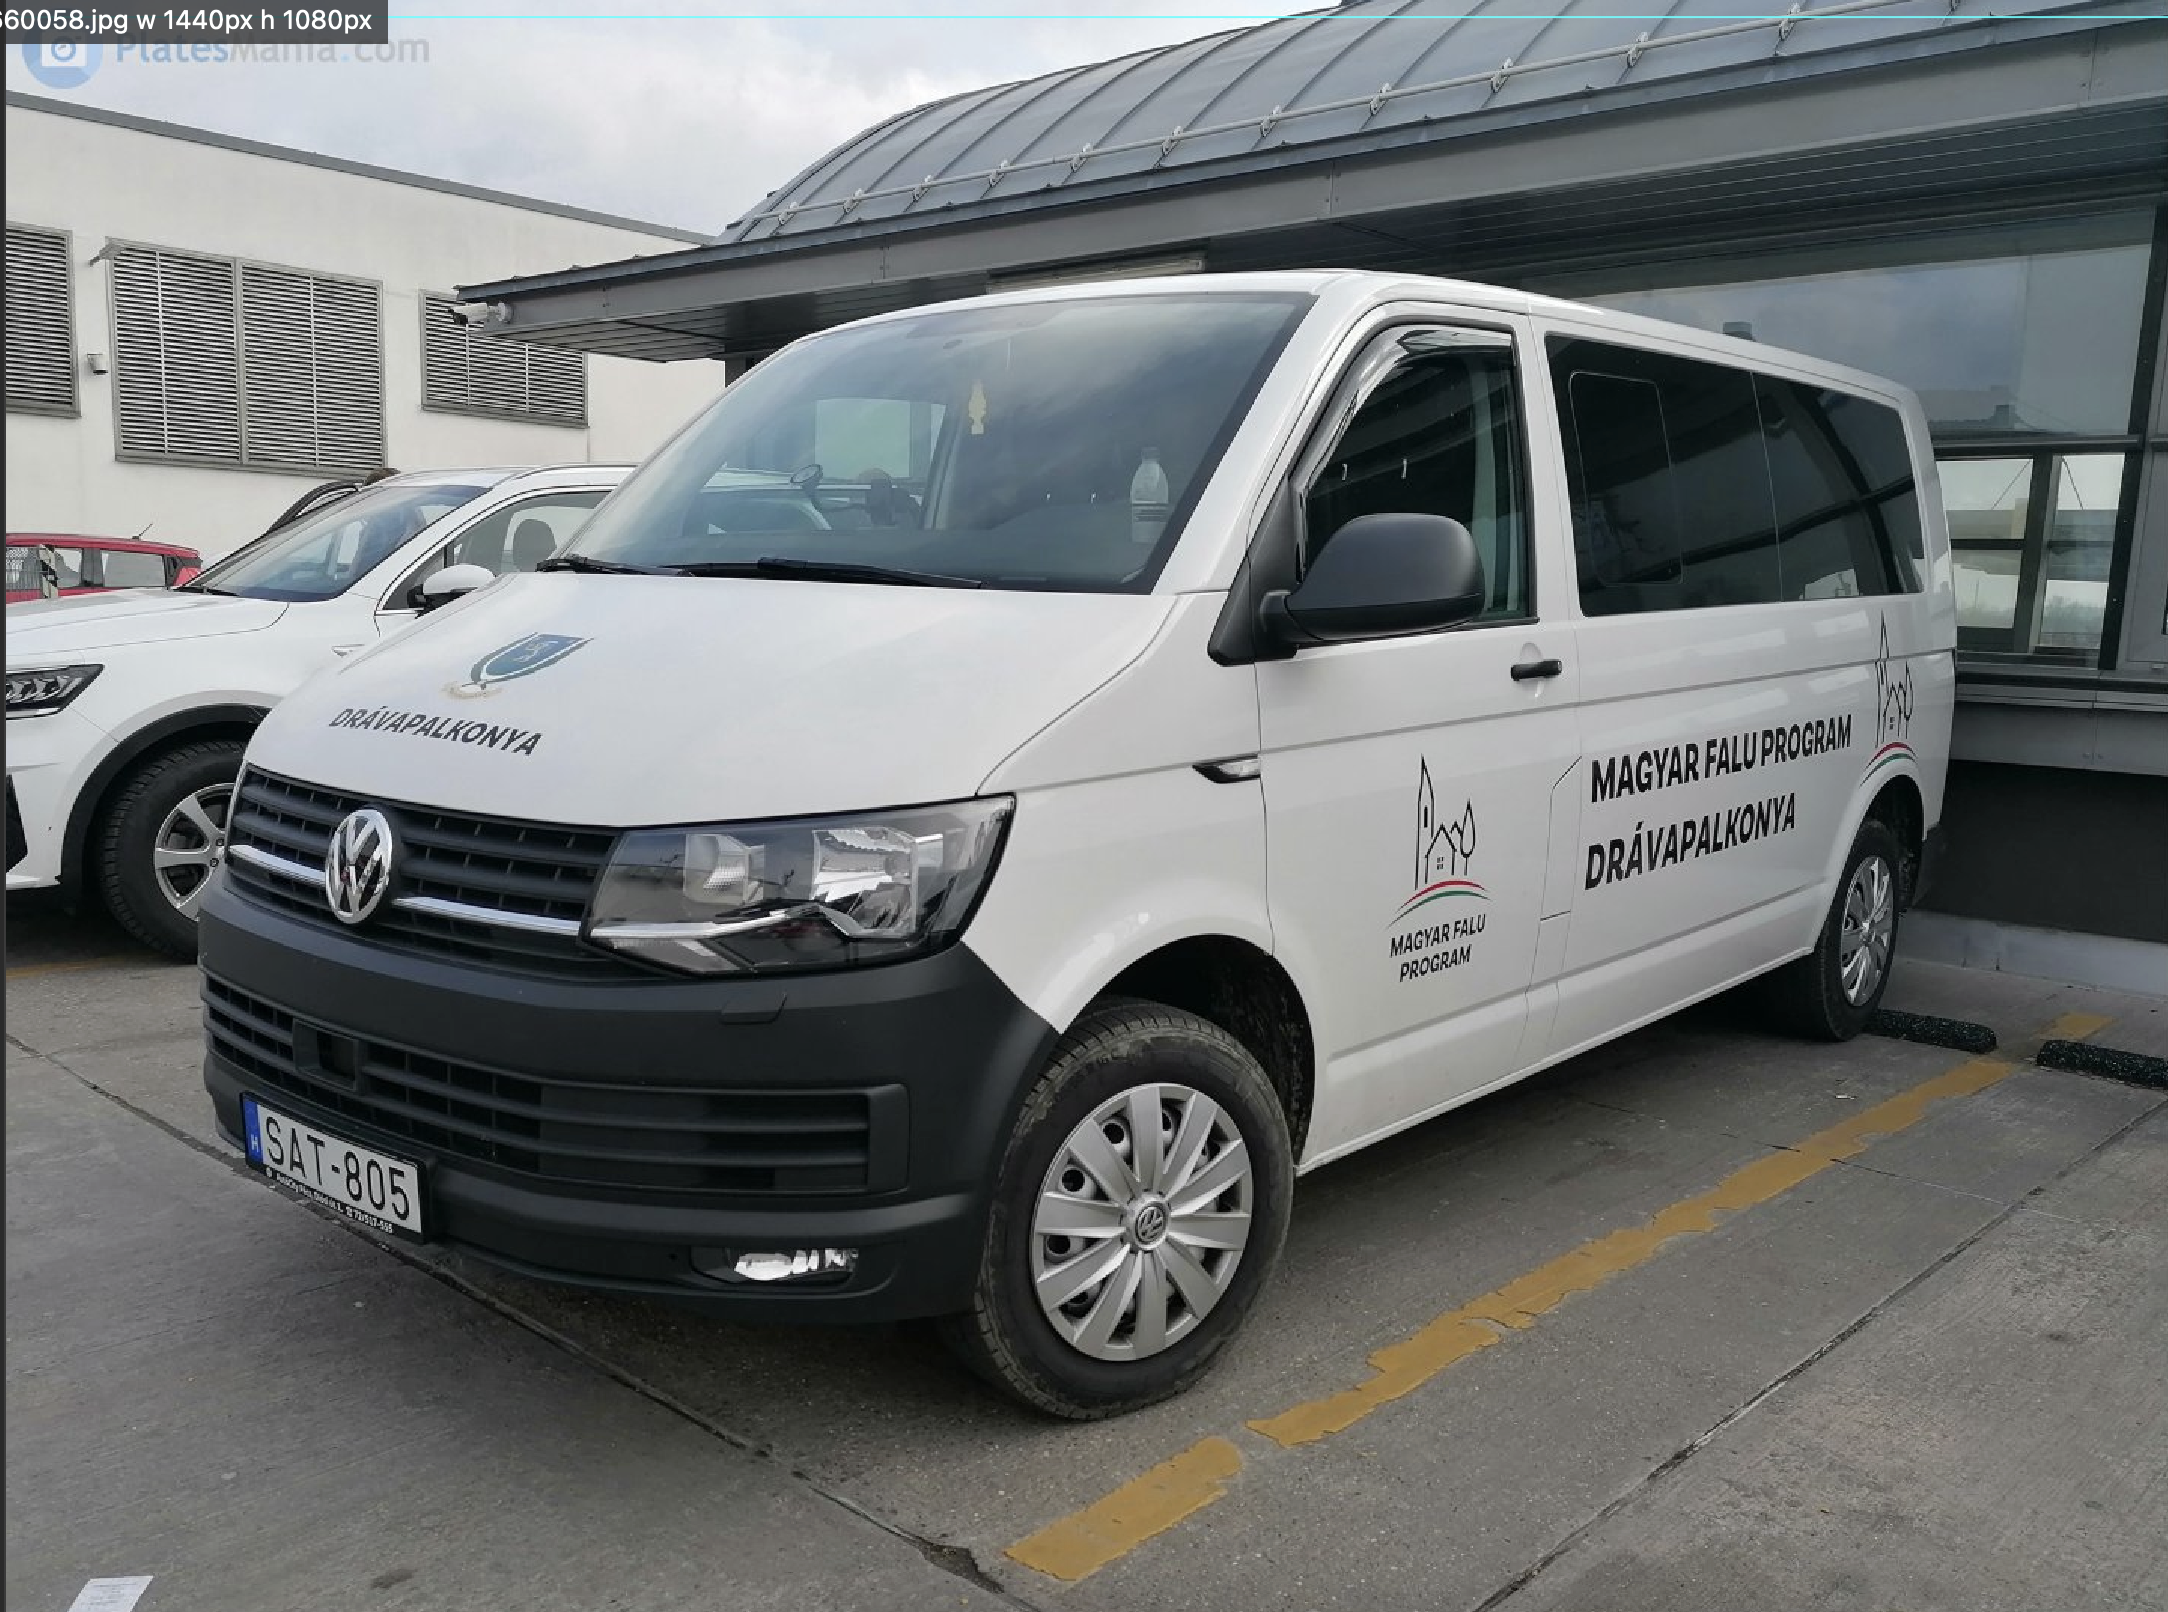
\includegraphics[height=.6\textwidth]{images/wrong_annotation.png}

		\textbf{Nincs annotálás}
	\end{minipage}\begin{minipage}{.5\textwidth}
		\centering
		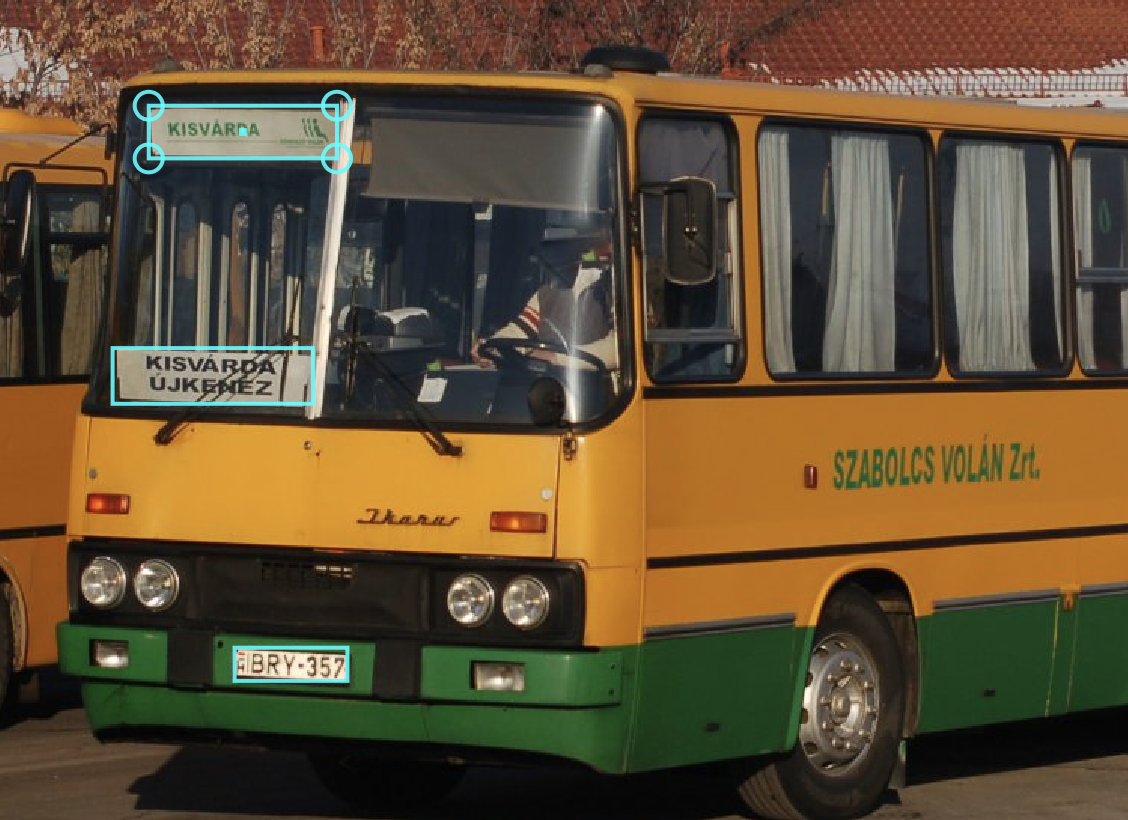
\includegraphics[height=.6\textwidth]{images/no_annotation.png}

		\textbf{Hibás annotálás}
	\end{minipage}
\end{frame}

\begin{frame}[fragile]
	\frametitle{5. lépés: YOLO betanítása a teljes képadatbázison}

	\begin{minted}[fontsize=\footnotesize]{python}
model.train(
    data='datasets/data_manual_v2.yaml',
    epochs=100,                       
    imgsz=512,                        
    batch=32,                         
    device="mps",                     
    workers=8,                        
    cache=True,                       
    augment=True,                     
    name='yolov8n_manual_train',      
    optimizer='AdamW',                
    lr0=1e-3,                         
    lrf=0.01,                         
    weight_decay=1e-2,                
    patience=10,                      
    seed=42,                          
)
\end{minted}

\end{frame}

\subsection{Rendszámtábla karakterek detekciója}
\begin{frame}
	\frametitle{OCR \texttt{fast-plate-ocr} segítségével}

	\begin{itemize}
		\item Nyílt forráskódú OCR modell, kifejezetten rendszámtáblák karaktereinek felismerésére fejlesztve
		\item A YOLO által detektált rendszámtábla kivágása kerül bemenetként a modellhez
		\item \textbf{Előfeldolgozás:}
		      \begin{itemize}
			      \item Szürkeárnyalatos konvertálás, kontraszt javítás
			      \item Kép méretezése a modell elvárásai szerint
		      \end{itemize}
		\item \textbf{Kimenet:} Prediktált karakterek sorrendje és bizonytalansága
	\end{itemize}
\end{frame}

\section{Eredmények}
\begin{frame}[fragile]
	\frametitle{Mappában lévő képek detekciója}
	\begin{minipage}{.33\textwidth}
		\centering
		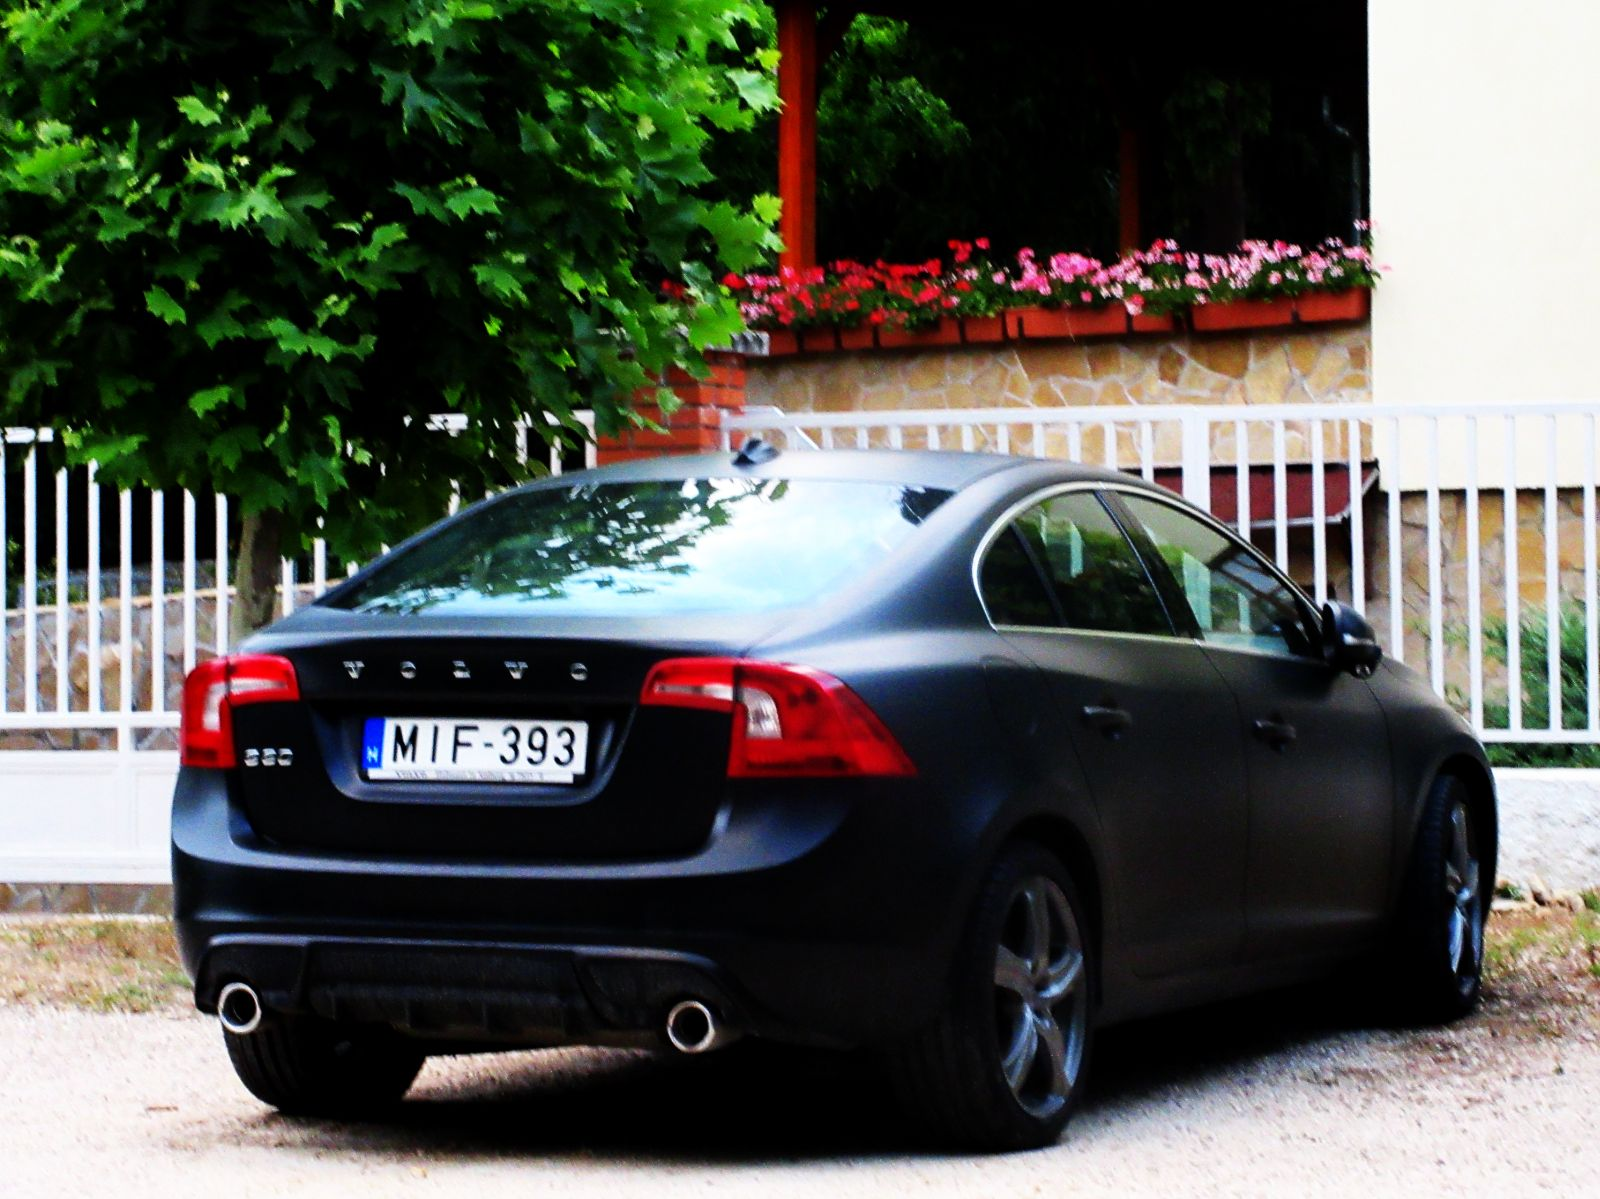
\includegraphics[height=.6\textwidth]{images/test-img-1.jpg}\\
		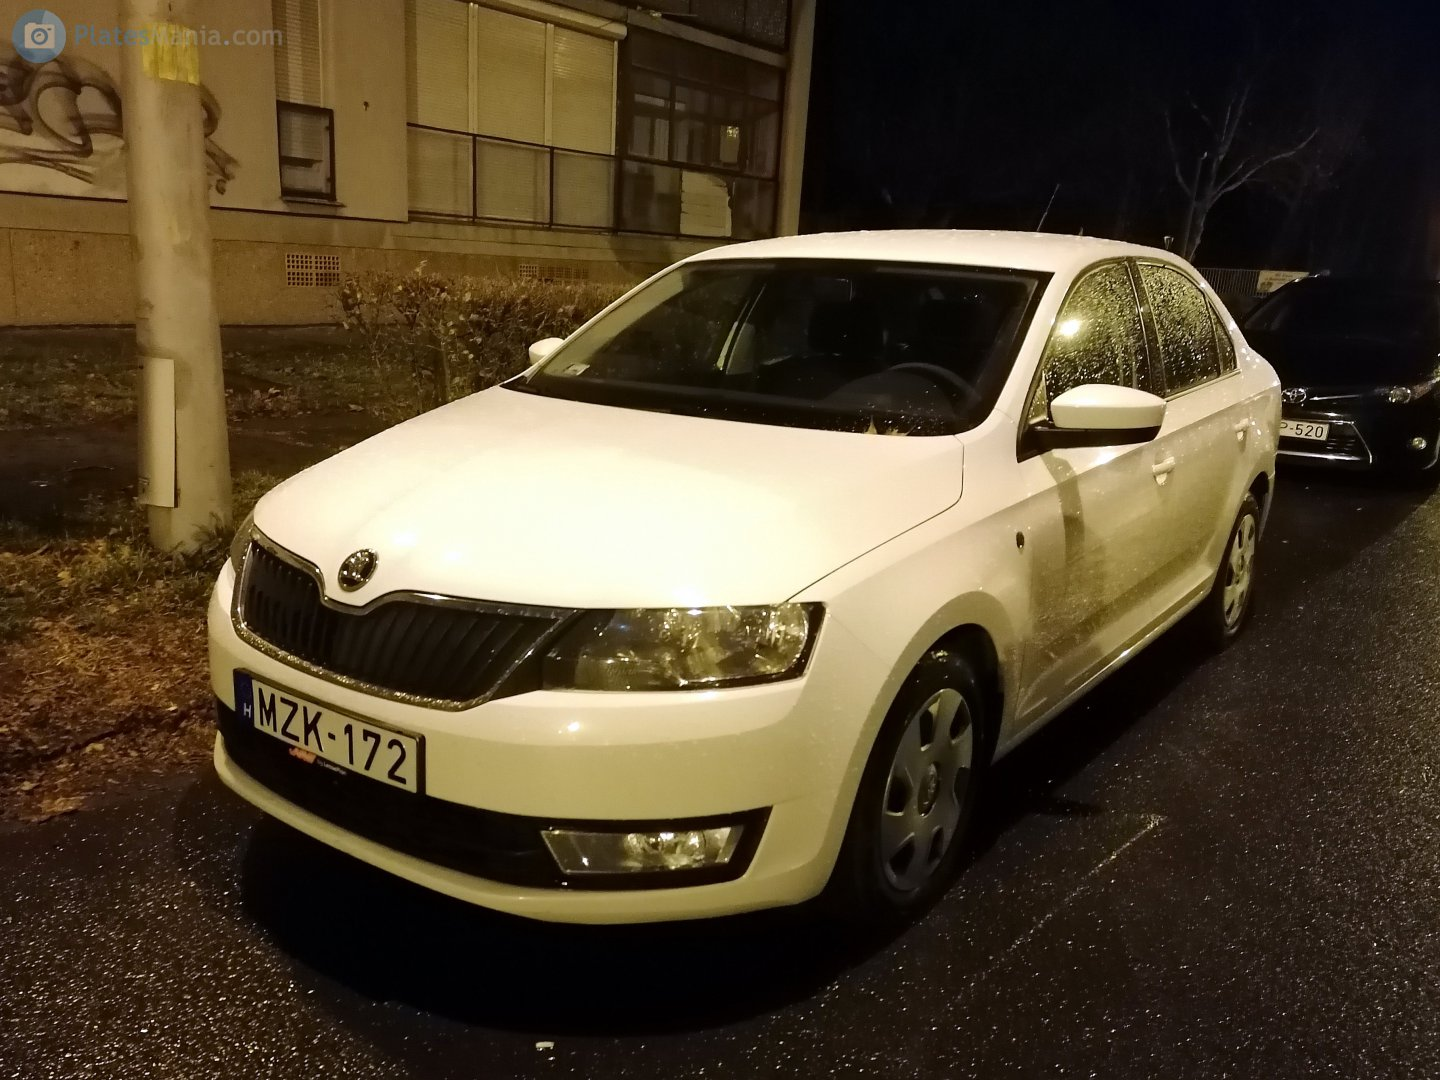
\includegraphics[height=.6\textwidth]{images/test-img-2.jpg}
	\end{minipage}\begin{minipage}{.33\textwidth}
		\centering
		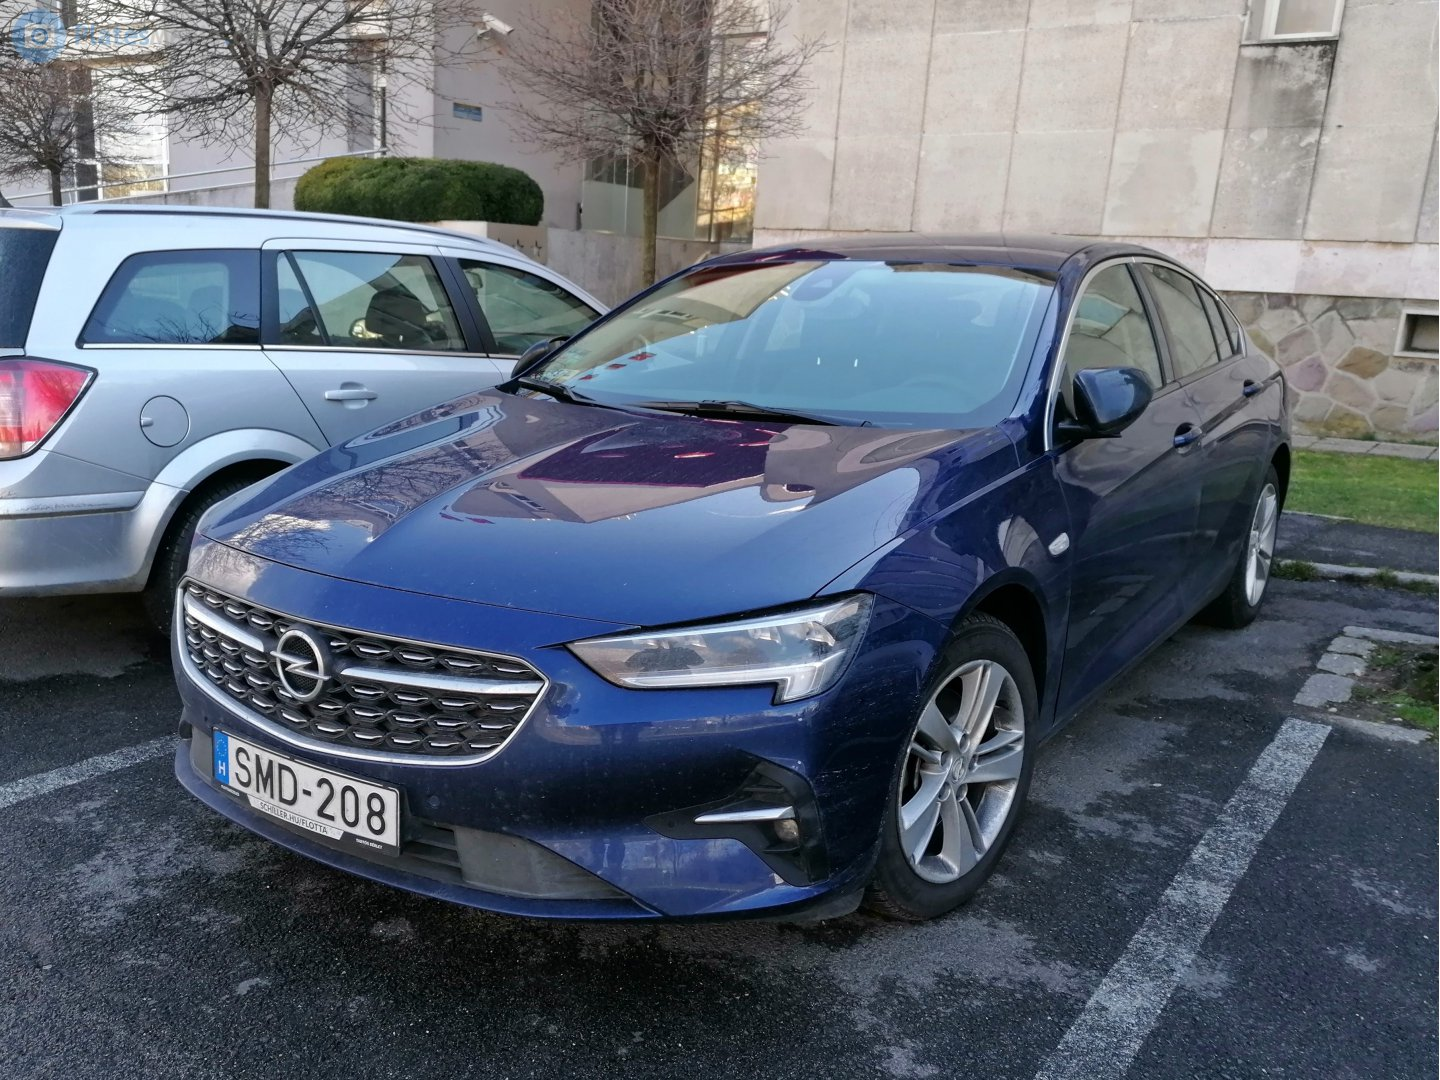
\includegraphics[height=.6\textwidth]{images/test-img-3.jpg}\\
		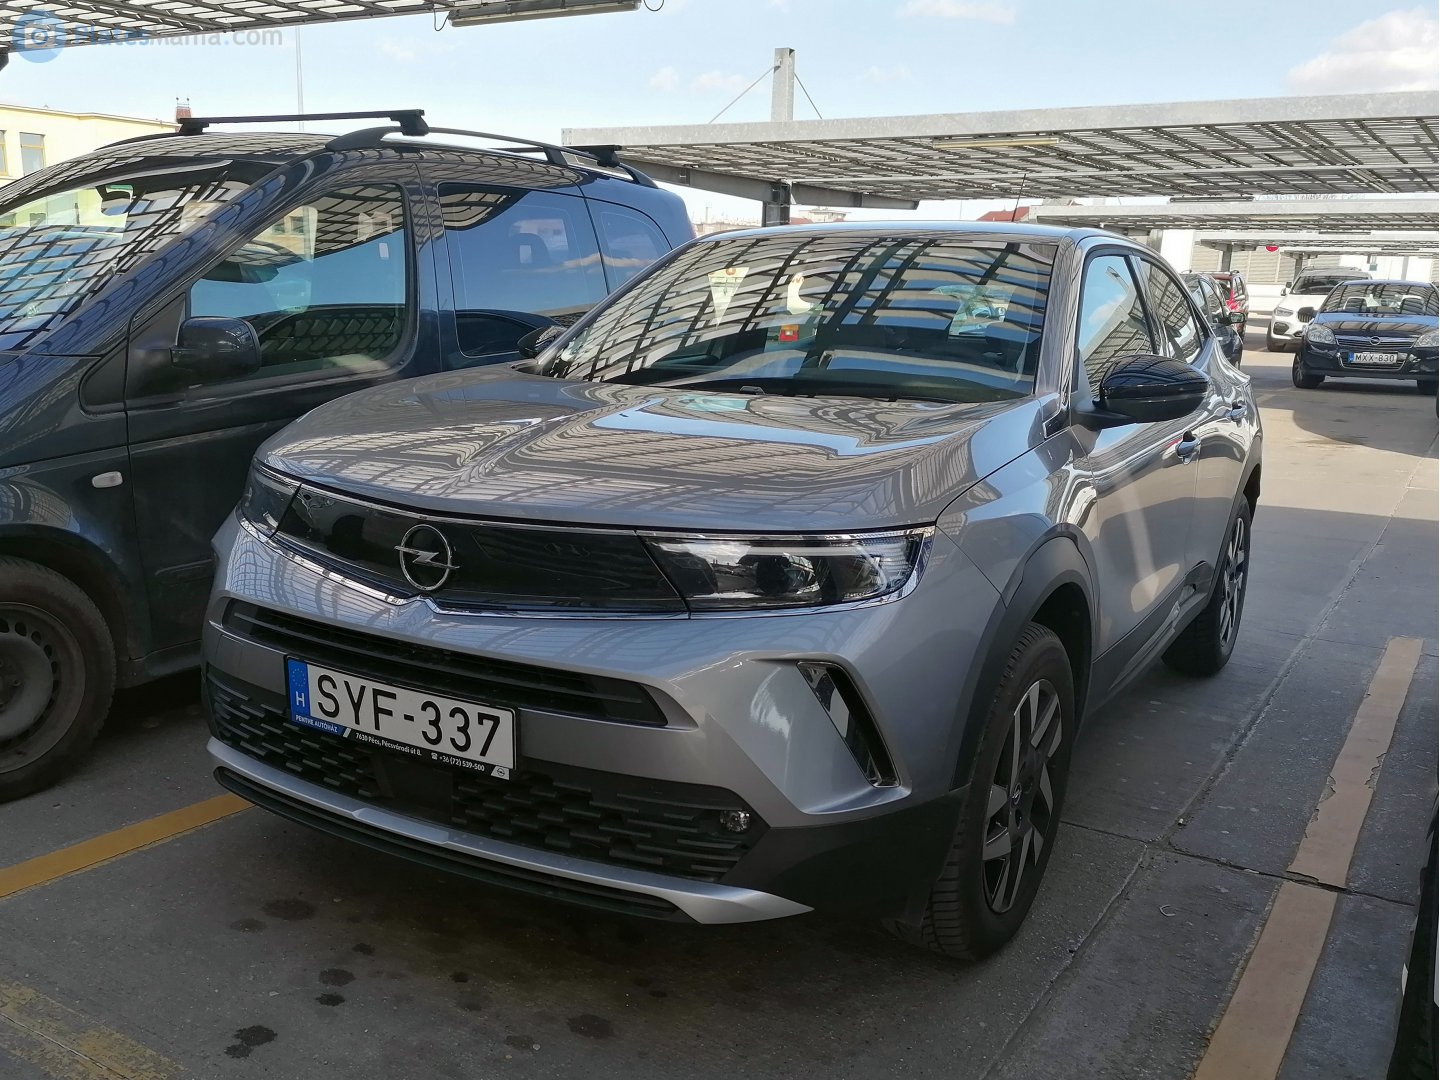
\includegraphics[height=.6\textwidth]{images/test-img-4.jpg}
	\end{minipage}\begin{minipage}{.33\textwidth}
		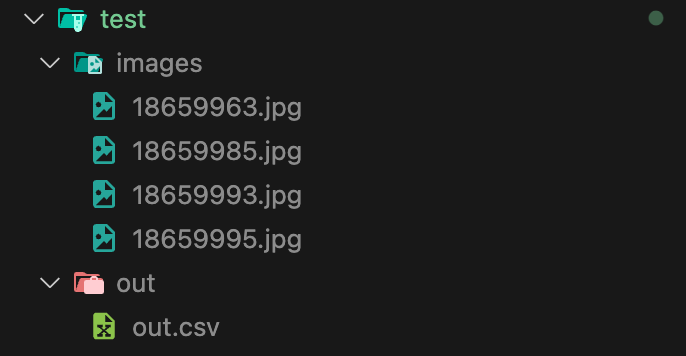
\includegraphics[height=.6\textwidth]{images/test_folder.png}

		\begin{minted}{text}
18659995.jpg;SYF-337
18659985.jpg;MZK-172
18659993.jpg;SMD-208
18659963.jpg;MIF-393
		\end{minted}
	\end{minipage}
\end{frame}

\begin{frame}
	\frametitle{Webes felület}

	\begin{minipage}{.5\textwidth}
		\centering
		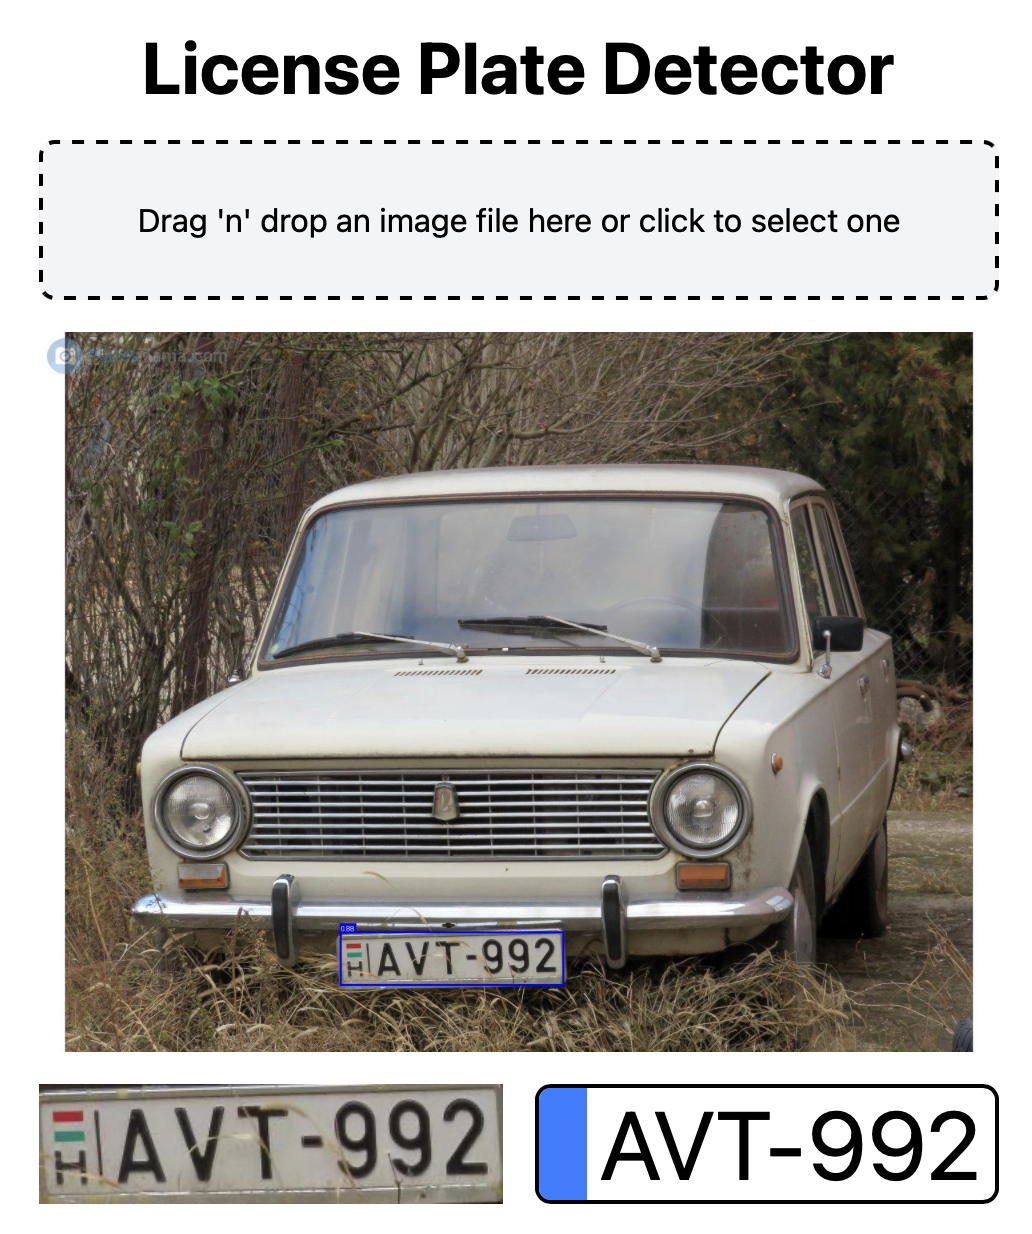
\includegraphics[height=.8\textwidth]{images/web_single.png}
	\end{minipage}\begin{minipage}{.5\textwidth}
		\centering
		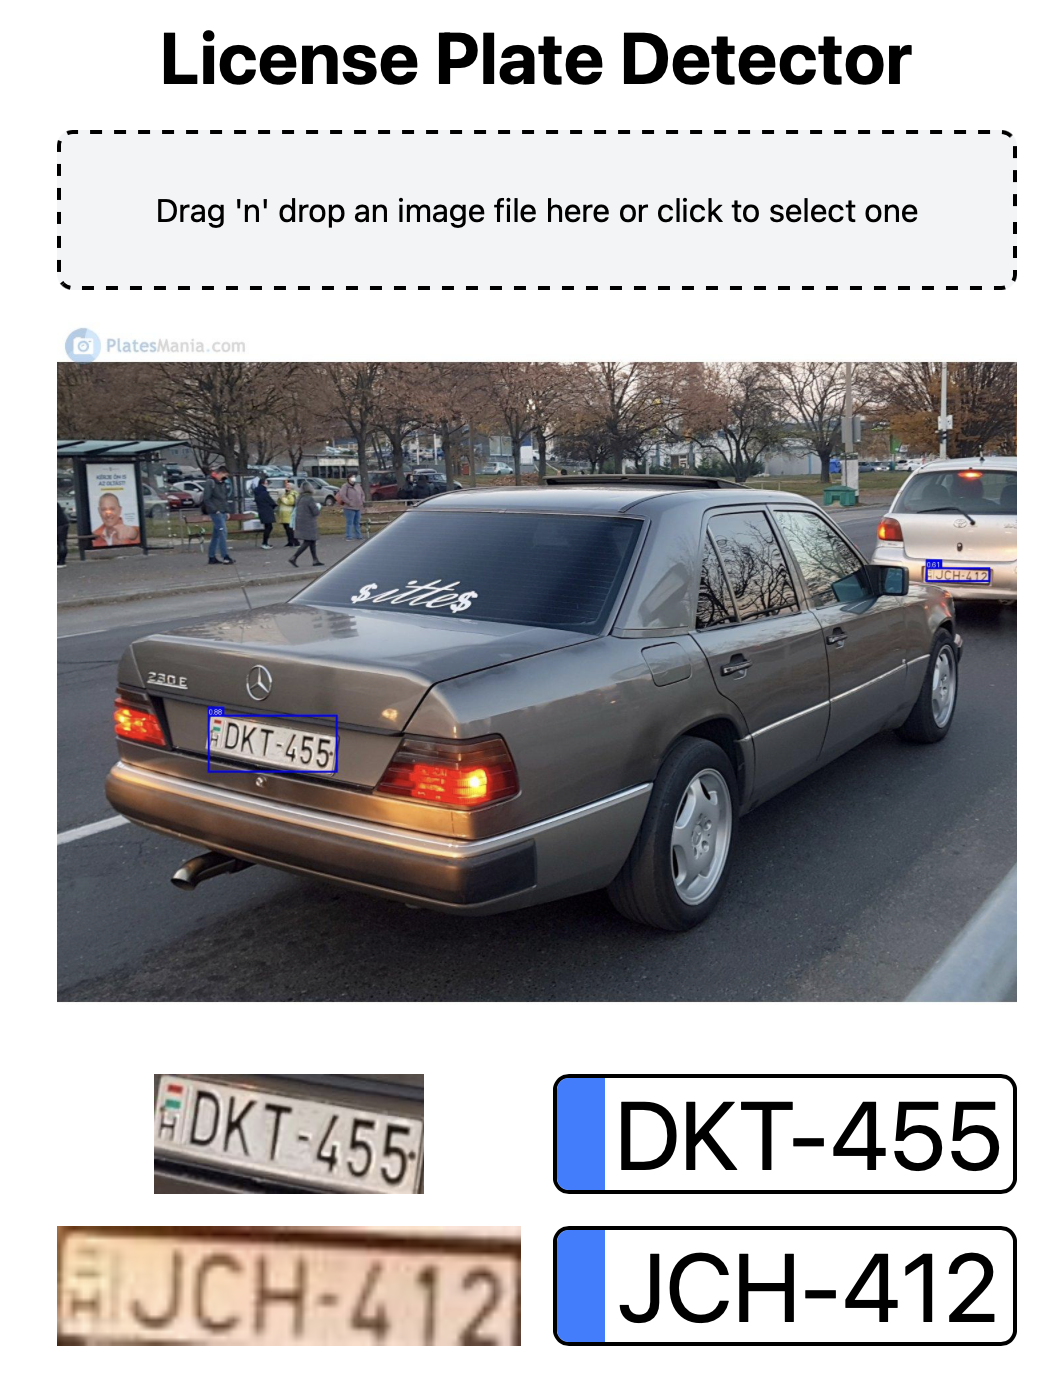
\includegraphics[height=.8\textwidth]{images/web_double.png}
	\end{minipage}
\end{frame}

\begin{frame}
	\Huge\bfseries
	\centering
	Köszönjük a figyelmet!
\end{frame}

\end{document}